\chapter{Spinors: Spin 1/2 Fields}
\section{Dirac's Approach to RQM:}
Dirac's primary goal was a 1st order relativistic Schrodinger equation, and he postulated that if it existed, it must have the general form of 
\begin{equation}
i \frac{\partial}{\partial t}|\psi\rangle= H|\psi\rangle=(a \cdot \mathbf{p}+\beta m)|\psi\rangle
\label{1st-order-relativistic-SDE}
\end{equation}
In \ref{1st-order-relativistic-SDE}, $\mathbf{p}$ is particle three momentum (an operator in quantum theories), and the vector $\alpha$ and the scalar $\beta$ would have to be determined. Thus, the equation would be first order in the time derivative. To find $\alpha$ and $\beta$, Dirac reasoned that $H^{2}$ and $|\psi\rangle$ must also satisfy the usual relativistic energy momentum relation (and therefore the Klein-Gordon equation)
$$
-\frac{\partial^{2}}{\partial t^{2}}|\psi\rangle= H^{2}|\psi\rangle=\left(\mathbf{p}^{2}+m^{2}\right)|\psi\rangle
$$
Thus
$$
-\frac{\partial^{2}}{\partial t^{2}}|\psi\rangle= H^{2}|\psi\rangle=\left(\alpha_{i} p_{i}+\beta m\right)\left(\alpha_{j} p_{j}+\beta m\right)|\psi\rangle
$$
$$
=\left(\alpha_{i}^{2} p_{i}^{2}+\underbrace{\left(\alpha_{i} \alpha_{j}+\alpha_{j} \alpha_{i}\right)}_{\text {must }=0}p_{i}p_{j}+\underbrace{\left(\alpha_{i} \beta+\beta \alpha_{i}\right)}_{\text {must }=0} p_{i} m+\beta^{2} m^{2}\right)|\psi\rangle
$$
Therefore, $\alpha_{i}^{2}=1$ and $\beta^{2}=1$. In summary, we have anti-commutators relationship:
\begin{qt}
    \begin{equation}
\begin{aligned}
&\left[\alpha_{i}, \alpha_{j}\right]_{+}=\left[\alpha_{i}, \beta\right]_{+}=0 \quad i \neq j \quad \alpha_{1}, \alpha_{2}, \alpha_{3}, \beta \text { all anti-commute with each other, }\\
&\left(\alpha_{1}\right)^{2}=\left(\alpha_{2}\right)^{2}=\left(\alpha_{3}\right)^{2}=(\beta)^{2}=1 \text { (the identity matrix) }
\end{aligned}
\label{standard-condition}
\end{equation}
\end{qt}
\bluep{If $\alpha_{i}$ and $\beta$ were numbers they would have to commute and could not possibly anti-commute. Hence, they can only be matrices. since these matrices are operators operating on $|\psi\rangle,$ then $|\psi\rangle$ itself must be a multicomponent object (i.e., a column matrix, at least.)}. Use the relations above, one can show that the \redp{$\alpha$ and $\beta$ matrices are traceless, hermitian, have $\pm$ eigenvalues, and must have an even dimension of at least four}.

Square matrices in a 4D space must be  $4\mathrm{X} 4,$ and thus if $|\psi\rangle$ is a column matrix (a vector), it must have four components (a 4D vector). Take care to note the \bluep{4D space we are talking about here is not the four-dimensional physical space of relativity theory, but an abstract pace, often called \textbf{spinor space}}.
\subsection{Standard presentation}
Choosing the minimum dimension case (four), Dirac and Pauli came up with a set of matrices which solve all of the conditions in (\ref{standard-condition}):
$$
\beta=\left[\begin{array}{cccc}
{1} \\
{} & {1} \\
{} & {} & {-1} \\
{} & {} & {} & {-1}
\end{array}\right]
$$
$$
\alpha_{1}=\left[\begin{array}{cccc}
{}&{}&{}&{1} \\
{}&{}&{1} \\
{} & {1} \\
{1}
\end{array}\right] \quad \alpha_{2}=\left[\begin{array}{cccc}
{}&{}&{}&{-i} \\
{}&{}&{i} \\
{} & {-i} \\
{i}
\end{array}\right] \quad \alpha_{3}=\left[\begin{array}{cccc}
{}&{}&{1} \\
{}&{}&{}& {-1} \\
{1}\\
{}&{-1} 
\end{array}\right]
$$
which are commonly written using Pauli matrices
$$
\beta=\left[\begin{array}{cc}
{I} & {0} \\
{0} & {-I}
\end{array}\right] \quad \alpha_{1}=\left[\begin{array}{cc}
{0} & {\sigma_{1}} \\
{\sigma_{1}} & {0}
\end{array}\right] \quad \alpha_{2}=\left[\begin{array}{cc}
{0} & {\sigma_{2}} \\
{\sigma_{2}} & {0}
\end{array}\right] \quad \alpha_{3}=\left[\begin{array}{cc}
{0} & {\sigma_{3}} \\
{\sigma_{3}} & {0}
\end{array}\right]
$$
If we define \textbf{gamma matrices} or \redp{\textbf{Dirac matrices}} as:
\begin{equation}
\gamma^{0}=\beta \quad \gamma^{1}=\beta \alpha_{1} \quad \gamma^{2}=\beta \alpha_{2} \quad \gamma^{3}=\beta \alpha_{3}
\end{equation}
we find the \textbf{Hermiticity conditions} as
\begin{equation}
\gamma^{\mu \dagger}=\gamma^{0} \gamma^{\mu} \gamma^{0}
\end{equation}
\subsection{Dirac equation expressed with Dirac matrices}
Pre-multiplied $\beta$, Dirac's original $1^{st}$ order equation takes on the form
\begin{equation}
i \beta \frac{\partial}{\partial t}|\psi\rangle=\left(\beta \alpha_{i} p_{i}+\beta^{2} m\right) | \psi\rangle=\left(-i \gamma^{i} \frac{\partial}{\partial x^{i}}+m\right)|\psi\rangle
\end{equation}
or rearranged as what is formally called the \textbf{Dirac equation}:
\begin{equation}
\sum_{\eta=1}^{4}\left(\sum_{\mu=0}^{3} i\left(\gamma^{\mu}\right)_{\kappa \eta} \partial_{\mu}-m \delta_{\kappa \eta}\right)|\psi\rangle_{\eta}=0 \quad \kappa=1,2,3,4
\end{equation}
where we have written out the $4 \mathrm{X} 4$ spinor space indices in $\kappa$ and $\eta$. Note the Dirac equation is actually \textbf{four separate non-matrix equations}, one for each value of the index $\kappa$. And each of these equations entails a sum of matrix components (sum over $\mu$ ), each post multiplied by one of the four components (in $\eta$ index) of the column vector $|\psi\rangle$.
\begin{qt}
    The common way to write the Dirac equation is to hide the spinor space indices in $\kappa$ and $\eta$,
    \begin{equation}
\left(i \gamma^{\mu} \partial_{\mu}-m\right)|\psi\rangle= 0
\label{convenient-Dirac-eq}
\end{equation}
Another notation commonly used, which is the most streamlined of all, is
$$
\not \partial=\gamma^{\mu} \partial_{\mu} \quad \text { so, the Dirac equation } \rightarrow(i \not \partial-m)|\psi\rangle= 0
$$
\end{qt}
Also, $m \rightarrow \frac{m c}{\hbar} \quad$ in non-natural units in the Dirac equation.

\subsection{Solutions to the Dirac equation}
Write out (\ref{convenient-Dirac-eq}) fully as:
$$
i \gamma^{\mu} \partial_{\mu}|\psi\rangle= i\left(\gamma^{0} \partial_{0}+\gamma^{1} \partial_{1}+\gamma^{2} \partial_{2}+\gamma^{3} \partial_{3}\right)|\psi\rangle= m|\psi\rangle=
$$
$$
=i\left(\left[\begin{array}{cccc}
{\partial_{0}} & {0} & {\partial_{3}} & {\partial_{1}-i \partial_{2}} \\
{0} & {\partial_{0}} & {\partial_{1}+i \partial_{2}} & {-\partial_{3}} \\
{-\partial_{3}} & {-\partial_{1}+i \partial_{2}} & {-\partial_{0}} & {0} \\
{-\partial_{1}-i \partial_{2}} & {\partial_{3}} & {0} & {-\partial_{0}}
\end{array}\right]\right) \left| \begin{array}{l}
{\psi_{1}} \\
{\psi_{2}} \\
{\psi_{3}} \\
{\psi_{4}}
\end{array}\right\rangle=
m\left|\begin{array}{l}
{\psi_{1}} \\
{\psi_{2}} \\
{\psi_{3}} \\
{\psi_{4}}
\end{array}\right\rangle
$$
The Dirac equation solutions in the Dirac-Pauli (standard) representation are
\begin{qt}
$$
\left|\psi^{(1)}\right\rangle=\sqrt{\frac{E+m}{2 m}}\left(\begin{array}{c}
{1} \\
{0} \\
{\frac{p^{3}}{E+m}} \\
{\frac{p^{1}+i p^{2}}{E+m}}
\end{array}\right)  \underbrace{e^{-i p x}}_{\text {4D physical space part}}=u_1e^{-i p x}
$$
$$
\left|\psi^{(2)}\right\rangle=\sqrt{\frac{E+m}{2 m}}\left(\begin{array}{c}
{0} \\
{1} \\
{\frac{p^{1}-i p^{2}}{E+m}} \\
{\frac{-p^{3}}{E+m}}
\end{array}\right) e^{-i p x}=u_2e^{-i p x}
$$
$$
\left|\psi^{(3)}\right\rangle=\sqrt{\frac{E+m}{2 m}}\left(\begin{array}{c}
{\frac{p^{3}}{E+m}} \\
{\frac{p^{1}+i p^{2}}{E+m}}\\
{1} \\
{0} 
\end{array}\right) e^{i p x}=v_2e^{i p x}
$$
\begin{equation}
\left|\psi^{(4)}\right\rangle=\sqrt{\frac{E+m}{2 m}}\left(\begin{array}{c}
{\frac{p^{1}-i p^{2}}{E+m}}\\
{\frac{-p^{3}}{E+m}} \\
{0} \\
{1} 
\end{array}\right) e^{i p x}=v_1e^{i p x}
\label{four-spinors}
\end{equation}
\end{qt}
We have defined new symbols $u_{r}(\mathbf{p})$ and $v_{r}(\mathbf{p})(r=1,2),$ which are the column vectors multiplied by the constant shown, are functions only of $\mathbf{p}$ for a given $m(\text { since } E=\sqrt{\mathbf{p}^{2}+m^{2}}),$ and go by the name \textbf{spinors}, or \textbf{\redp{four-spinors}}. Note that \bluep{the particles represented by $|\psi^{(n)}\rangle$ are also often called spinors.}

\textbf{$u_{1}$ represents spin up, and $u_{2}$ represents spin down in the particle at-rest system. As you might expect, we will find the solutions containing $v_{r}(\mathbf{p})$ are associated with antiparticles; and those with $u_{r}(\mathbf{p}),$ with particles.}\redp{Take care to note the reverse order numbering on $v_{2,1}$ from $u_{1,2},$ which is customary.}

If we take \textbf{inner products of four spinors}, we have
$$
u_{1}^{\dagger}(\mathbf{p}) u_{1}(\mathbf{p})=\frac{E}{m}
$$
More generally
\begin{equation}
u_{\underline{r}L}^{\dagger}(\mathbf{p}) u_{\underline{r}}(\mathbf{p})=v_{\underline{r}}^{\dagger}(\mathbf{p}) v_{\underline{r}}(\mathbf{p})=\frac{E}{m}
\end{equation}
Where underline means no summation. Also, spinors are \textbf{orthogonal}
\begin{equation}
\begin{aligned}
&u_{r}^{\dagger}(\mathbf{p}) u_{s}(\mathbf{p})=v_{r}^{\dagger}(\mathbf{p}) v_{s}(\mathbf{p})=\frac{E}{m} \delta_{r s}\\
&u_{r}^{\dagger}(\mathbf{p}) v_{s}(-\mathbf{p})=0
\end{aligned}
\end{equation}
Therefore, the eigensolutions are also orthogonal
\begin{equation}
\left\langle\psi^{(m)} | \psi^{(n)}\right\rangle= 0 \text { for } m \neq n
\end{equation}
For example
$$
\left\langle\psi^{(1)} | \psi^{(3)}\right\rangle=\int u_{1}^{\dagger}(\mathbf{p}) e^{+i p x} v_{2}(\mathbf{p}) e^{+i p x} d^{3} x=\underbrace{u_{1}^{\dagger}(\mathbf{p}) v_{2}(\mathbf{p})}_{=0 \text { for } \mathbf{p}=0} \underbrace{\int e^{+i p x} e^{+i p x} d^{3} x}_{=0 \text { for } \mathbf{p} \neq 0}=0
$$
where we follow \textbf{Cesaro integration}:$\int_{0}^{\infty} \sin x d x=1$ and $\int_{0}^{\infty} \cos x d x=0$.
\begin{qt}
The most general solution to the Dirac equation is:
\begin{equation}
\psi_{\text {state}}=|\psi\rangle=\sum_{r, \mathbf{p}} \sqrt{\frac{m}{V E_{\mathrm{p}}}}\left(C_{r}(\mathbf{p}) u_{r}(\mathbf{p}) e^{-i p x}+D_{r}^{\dagger}(\mathbf{p}) v_{r}(\mathbf{p}) e^{i p x}\right)
\label{general-Dirac-state}
\end{equation}
Unlike the Klein-Gordon equation, the Dirac equation is a matrix equation. So, rather than complex conjugate form of the wave equation, we need to consider \textbf{taking a complex conjugate pose of that equation}, we define  and use the \textbf{adjoint}
\begin{equation}
\bar{\psi}_{\text {state}}=\psi_{\text {state}}^{\dagger} \gamma^{0}=|\psi\rangle^{\dagger} \gamma^{0}=\left\langle\psi\left|\gamma^{0}=\langle\bar{\psi}|\right.\right.
\end{equation}
\redp{where an inner product between the row vector $|\psi\rangle^{\dagger}=\langle\psi|=\psi^{+}$ state and the gamma matrix are implied.} The adjoint Dirac equation is
\begin{equation}
i \partial_{\mu}\left\langle\bar{\psi}\left|\gamma^{\mu}+m\langle\bar{\psi}|=0\right.\right.
\label{adjoint-Dirac-eq}
\end{equation}
\end{qt}
Adjoint spinors are defined as the row vectors
\begin{equation}
\bar{u}_{r}=u_{r}^{\dagger} \gamma^{0} \quad \bar{v}_{r}=v_{r}^{\dagger} \gamma^{0}
\end{equation}
which, gives us the \textbf{\underline{discrete plane wave adjoint general solution form}}:
\begin{equation}
\bar{\psi}_{\text {state}}=\langle\bar{\psi}|=\sum_{r, \mathrm{p}} \sqrt{\frac{m}{V E_{\mathrm{p}}}}\left(D_{r}(\mathrm{p}) \bar{v}_{\mathrm{r}}(\mathrm{p}) e^{-i p x}+C_{r}^{\dagger}(\mathrm{p}) \bar{u}_{r}(\mathrm{p}) e^{i p x}\right)
\end{equation}
\subsection{Probability density for Dirac Fermions}
The \textbf{four-current} using the Dirac equation can be found to be
\begin{qt}
\begin{equation}
\partial_{\mu} j^{\mu}=0 \quad j^{\mu}=(\rho, \mathbf{j})=\bar{\psi}_{\text {state }} \gamma^{\mu} \psi_{\text {state }}=\left\langle\bar{\psi}\left|\gamma^{\mu}\right| \psi\right\rangle_{\text {not integ }}
\label{four-current-Dirac}
\end{equation}
where the subscript "not intg" means we are not integrating over space in the bracket shown.
\end{qt}
The (\ref{four-current-Dirac}) means the total quantity
\begin{equation}
\begin{aligned}
\int_{V} j^{0} d^{3} x &=\int_{V} \rho d^{3} x=\int_{V} \bar{\psi}_{\text {state}} \gamma^{0} \psi_{\text {state}} d^{3} x=\left\langle\bar{\psi}\left|\gamma^{0}\right| \psi\right\rangle \\
&=\int_{V} \psi_{\text {state}}^{\dagger} \gamma^{0} \gamma^{0} \psi_{\text {state}} d^{3} x=\langle\psi | \psi\rangle= Q^{\prime}
\end{aligned}
\end{equation}
is conserved for $V$= all space. \textbf{For a single particle state in RQM, if we assume the solution onlu terms with coefficients $C_r$}(i.e., only has spinors of form $u_r$), our $\rho$ becomes
\begin{equation}
\begin{aligned}
\rho &\left.=\left(\sum_{r, p} \sqrt{\frac{m}{V E_{p}}} C_{r}^{\dagger}(p) \underbrace{\bar{u}_{r}(p)}_{u_{r}^{\dagger}(p) \gamma^{o}}\right)e^{i p x}\right) \gamma^{0}\left(\sum_{r^{\prime}, p^{\prime}} \sqrt{\frac{m}{V E_{p^{p}}}} C_{r^{\prime}}\left(p^{\prime}\right) u_{r^{\prime}}^{\prime}\left(p^{\prime}\right) e^{-i p^{\prime} x}\right) \\
&=\left(\sum_{r, p} \sqrt{\frac{m}{V E_{p}}} C_{r}^{\dagger}(p) u_{r}^{\dagger}(p) e^{i p x}\right)\left(\sum_{r^{\prime}, p^{\prime}} \sqrt{\frac{m}{V E_{p}}} C_{r^{\prime}}\left(p^{\prime}\right) u_{r^{\prime}}\left(p^{\prime}\right) e^{-i p^{\prime} x}\right)
\end{aligned}
\end{equation}
If this is probability density, we have
$$
\int \rho d^{3} x=\sum_{r, p} \frac{m}{V}\left(C_{r}^{\dagger}(\mathrm{p}) C_{r}(\mathrm{p}) \frac{u_{r}^{\dagger}(\mathbf{p}) u_{r}(\mathrm{p})}{E_{p} / m} \underbrace{\int e^{-i p x}e^{ip x}d^{3} x}_{V}\right)==\sum_{r, \mathrm{p}}\left|C_{r}(\mathrm{p})\right|^{2}=1
$$
\bluep{Notice that a Dirac fermion represented by a solution with exponential form $-ipx$(that has spinor $u_r$ and coefficient $C_r(\mathbf{p})$), has positive energy; and one represented by solution form $ipx$(spinor $v_{r}$ and coefficient $D_{r}^{\dagger}(\mathrm{p})$ ), has negative energy.}

\subsection{Dirac approach to Spin}
\redp{The RQM spin operator} are defined as:
\begin{qt}
\begin{equation}
 \Sigma_{1}=\frac{\hbar}{2}\left[\begin{array}{cccc}
{} & {1} & {} & {} \\
{1} & {} & {} & {} \\
{} & {} & {} & {1} \\
{} & {} & {1} & {}
\end{array}\right] \Sigma_{2}=\frac{\hbar}{2}\left[\begin{array}{cccc}
{} & {-i} & {} & {} \\
{i} & {} & {} & {} \\
{} & {} & {} & {-i} \\
{} & {} & {i} & {}
\end{array}\right] \Sigma_{3}=\frac{\hbar}{2}\left[\begin{array}{cccc}
{1} & {} & {} & {} \\
{} & {-1} & {} & {} \\
{} & {} & {1} & {} \\
{} & {} & {} & {-1}
\end{array}\right]
\label{RQM-spin-operators}
\end{equation}
\end{qt}
Note $\Sigma_i$ (\ref{RQM-spin-operators}) is a $3 \mathrm{D}$ object in physical space (3 components of the spin angular momentum), but \textbf{each of the components in that space is itself a $4 \mathrm{X} 4$ matrix in relativistic $4 \mathrm{D}$ spinor space, rather than non-relativistic 2 D spinor space of NRQM.} \redp{In relativity. spin has three spatial components. But, relativistically, each component must act on a $4 \mathrm{D}$ column vector in spinor space.}

Consider a stationary Dirac particle which has $\mathrm{p}=0$ in our frame, and the solutions (\ref{four-spinors}) become much simplified. What then, are their respective spins? For the first such solution, we have
$$
\Sigma_{3}\left|\psi^{(1)}\right\rangle=\frac{\hbar}{2}\left[\begin{array}{cccc}
{1} \\
{}&{-1} \\
{} & {} & {1}\\
{} &{} &{}& {-1}
\end{array}\right] \sqrt{\frac{m+m}{2 m}}\left(\begin{array}{l}
{1} \\
{0} \\
{0} \\
{0}
\end{array}\right) e^{-i p x}=\frac{\hbar}{2}\left(\begin{array}{l}
{1} \\
{0} \\
{0} \\
{0}
\end{array}\right) e^{-i p x}=\frac{\hbar}{2}\left|\psi^{(1)}\right\rangle
$$
Therefore \textbf{\underline{$\left|\psi^{(1)}\right\rangle$ is for spin up.}}

As soon as we have a moving particle, things get more complicated, as we have to include nonzero $p^{i}$ values in our solutions (\ref{four-spinors}) This complication, which we didn't have in $\mathrm{NRQM},$ is due to relativistic effects.
\begin{mybox}
\textbf{Classical Macroscopic Spinning Object Translating at Relativistic Speed}

In $4 \mathrm{D}$ relativistic theory, angular momentum is a $2^{\mathrm{nd}}$ order tensor, but it can be treated simply as a vector formed from the integral over a rotating body of $d m\left(\mathbf{r} \times \mathbf{v}_{t}\right)=d m(\mathbf{r} \times(\omega \times \mathbf{r})),$ where symbols should be obvious. When a macroscopic object like a spinning disk, as shown below, moves close to the speed of light, distances contract in the direction of the velocity, and this makes the plane of the disk appear to turn. (See figure below.)
\end{mybox}
\begin{figure}[H]
    \centering
    \tikzset{every picture/.style={line width=0.75pt}} %set default line width to 0.75pt        
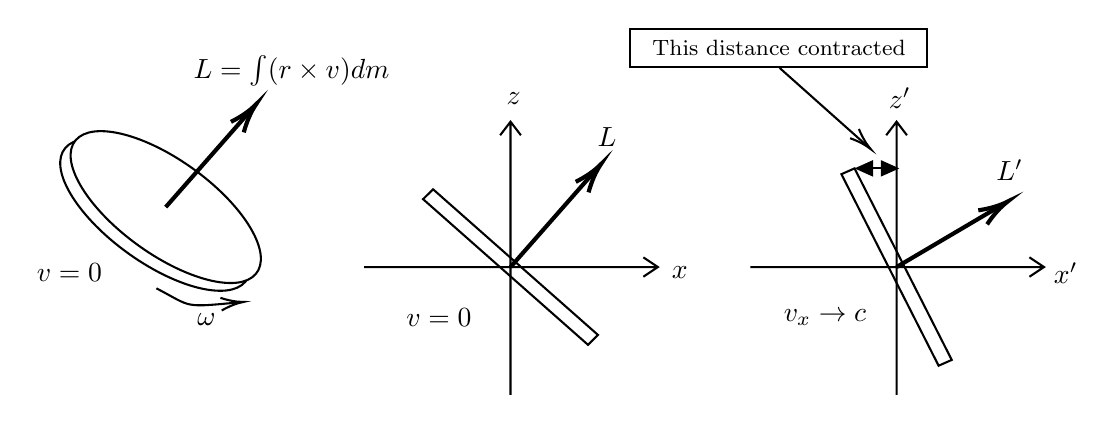
\begin{tikzpicture}[x=0.75pt,y=0.7pt,yscale=-1,xscale=1]
%uncomment if require: \path (0,300); %set diagram left start at 0, and has height of 300

%Shape: Ellipse [id:dp6696584947764774] 
\draw   (105.99,95.55) .. controls (114.14,85.31) and (140.18,92.46) .. (164.14,111.53) .. controls (188.1,130.6) and (200.92,154.36) .. (192.77,164.6) .. controls (184.62,174.85) and (158.58,167.7) .. (134.62,148.63) .. controls (110.66,129.56) and (97.84,105.8) .. (105.99,95.55) -- cycle ;
%Shape: Ellipse [id:dp8843951455763316] 
\draw  [fill={rgb, 255:red, 255; green, 255; blue, 255 }  ,fill opacity=1 ] (110.99,91.55) .. controls (119.14,81.31) and (145.18,88.46) .. (169.14,107.53) .. controls (193.1,126.6) and (205.92,150.36) .. (197.77,160.6) .. controls (189.62,170.85) and (163.58,163.7) .. (139.62,144.63) .. controls (115.66,125.56) and (102.84,101.8) .. (110.99,91.55) -- cycle ;
%Straight Lines [id:da6714691596952527] 
\draw [line width=1.5]    (154.38,126.08) -- (196,75.35) ;
\draw [shift={(197.9,73.03)}, rotate = 489.37] [color={rgb, 255:red, 0; green, 0; blue, 0 }  ][line width=1.5]    (14.21,-4.28) .. controls (9.04,-1.82) and (4.3,-0.39) .. (0,0) .. controls (4.3,0.39) and (9.04,1.82) .. (14.21,4.28)   ;

%Curve Lines [id:da608409716212424] 
\draw    (149.9,168.03) .. controls (167.54,177.83) and (162.13,178.03) .. (190.14,175.21) ;
\draw [shift={(191.9,175.03)}, rotate = 534.29] [color={rgb, 255:red, 0; green, 0; blue, 0 }  ][line width=0.75]    (10.93,-3.29) .. controls (6.95,-1.4) and (3.31,-0.3) .. (0,0) .. controls (3.31,0.3) and (6.95,1.4) .. (10.93,3.29)   ;

%Shape: Rectangle [id:dp2988248655701031] 
\draw  [fill={rgb, 255:red, 255; green, 255; blue, 255 }  ,fill opacity=1 ] (283.18,116.89) -- (362.64,192.09) -- (357.82,197.17) -- (278.36,121.98) -- cycle ;
%Shape: Axis 2D [id:dp3998228460871881] 
\draw [line width=0.75]  (250,157.03) -- (391.5,157.03)(320.5,82) -- (320.5,223.03) (384.5,152.03) -- (391.5,157.03) -- (384.5,162.03) (315.5,89) -- (320.5,82) -- (325.5,89)  ;
%Straight Lines [id:da08204495575914073] 
\draw [line width=1.5]    (320.5,157.03) -- (362.12,106.31) ;
\draw [shift={(364.02,103.99)}, rotate = 489.37] [color={rgb, 255:red, 0; green, 0; blue, 0 }  ][line width=1.5]    (14.21,-4.28) .. controls (9.04,-1.82) and (4.3,-0.39) .. (0,0) .. controls (4.3,0.39) and (9.04,1.82) .. (14.21,4.28)   ;

%Shape: Rectangle [id:dp9756203932975158] 
\draw  [fill={rgb, 255:red, 255; green, 255; blue, 255 }  ,fill opacity=1 ] (486.24,106.1) -- (533.08,204.97) -- (526.76,207.96) -- (479.92,109.1) -- cycle ;
%Shape: Axis 2D [id:dp2253494066411521] 
\draw [line width=0.75]  (436,157.03) -- (577.5,157.03)(506.5,82) -- (506.5,223.03) (570.5,152.03) -- (577.5,157.03) -- (570.5,162.03) (501.5,89) -- (506.5,82) -- (511.5,89)  ;
%Straight Lines [id:da26681235965231986] 
\draw [line width=1.5]    (506.5,157.03) -- (557.46,124.84) ;
\draw [shift={(560,123.23)}, rotate = 507.72] [color={rgb, 255:red, 0; green, 0; blue, 0 }  ][line width=1.5]    (14.21,-4.28) .. controls (9.04,-1.82) and (4.3,-0.39) .. (0,0) .. controls (4.3,0.39) and (9.04,1.82) .. (14.21,4.28)   ;

%Straight Lines [id:da2736459794596652] 
\draw    (489.24,106.1) -- (504.8,106.1) ;
\draw [shift={(507.8,106.1)}, rotate = 180] [fill={rgb, 255:red, 0; green, 0; blue, 0 }  ][line width=0.08]  [draw opacity=0] (8.93,-4.29) -- (0,0) -- (8.93,4.29) -- cycle    ;
\draw [shift={(486.24,106.1)}, rotate = 0] [fill={rgb, 255:red, 0; green, 0; blue, 0 }  ][line width=0.08]  [draw opacity=0] (8.93,-4.29) -- (0,0) -- (8.93,4.29) -- cycle    ;
%Straight Lines [id:da8576239603286319] 
\draw    (450.13,54.23) -- (492.69,94.85) ;
\draw [shift={(494.13,96.23)}, rotate = 223.67000000000002] [color={rgb, 255:red, 0; green, 0; blue, 0 }  ][line width=0.75]    (10.93,-3.29) .. controls (6.95,-1.4) and (3.31,-0.3) .. (0,0) .. controls (3.31,0.3) and (6.95,1.4) .. (10.93,3.29)   ;


% Text Node
\draw (174,184) node    {$\omega $};
% Text Node
\draw (108,160) node    {$v=0$};
% Text Node
\draw (402,160) node    {$x$};
% Text Node
\draw (322,70) node    {$z$};
% Text Node
\draw (215,56) node    {$L=\int ( r\times v) dm$};
% Text Node
\draw (367,90) node    {$L$};
% Text Node
\draw (286,183) node    {$v=0$};
% Text Node
\draw (588,160) node    {$x'$};
% Text Node
\draw (508,70) node    {$z'$};
% Text Node
\draw (561,107) node    {$L^{\prime }$};
% Text Node
\draw (472,183) node    {$v_{x}\rightarrow c$};
% Text Node
\draw    (378,34) -- (521,34) -- (521,54) -- (378,54) -- cycle  ;
\draw (449.87,44) node  [font=\footnotesize] [align=left] {This distance contracted};


\end{tikzpicture}
    \caption{Spinning disk}
    \label{fig:spinning-disk}
\end{figure}
The closer the disk gets to the speed of light, the more the disk surface appears in the observer's frame to align normal to the velocity direction. In the rest frame translating with the disk itself, the disk still appears aligned in the original way. In the observer's frame, though, the angular momentum L appears to turn toward the direction of the velocity becoming $L^{\prime}$. The greater the speed, the greater this turning. At light speed, $L^{\prime}$ and $v$ become parallel.

Quantum mechanically, then, \bluep{at high speed, a particle's angular momentum (spin) magnitude remains unchanged, but its direction appears to us in our frame to realign itself closer to that of the translational velocity vector.}

Mathematically, these kinds of relativistic complications are incorporated into the form of the spinors $u_{r}(\mathrm{p})$ and $v_{r}(\mathrm{p})$ (by their dependence on 3 -momentum and thus ultimately, on velocity) and by how they are combined to form more general spin states.

\begin{qt}
\redp{Note that the spinor components are actually dependent on particle velocity, rather than momentum, by the following logic.} Energy and momentum are expressed (in non-natural units to make it easier to understand)
$$
E=\frac{m c^{2}}{\sqrt{1-v^{2} / c^{2}}} \quad p^{i}=\frac{m v^{i}}{\sqrt{1-v^{2} / c^{2}}}
$$
so in the coefficient and spinor components of the Dirac spinor (\ref{four-spinors}) the mass $m$ drops out. This leaves them a function solely of velocity.
\end{qt}

\subsubsection{What happens when the particle is not stationary}
Note what happens to the spin as seen by us, for an electron whose spin is represented solely by
$u_{1},$ but has $p^{1} \neq 0,$ with $p^{2}=p^{3}=0$ in our frame (the lab.)
$$
\Sigma_{3}\left|\psi^{(1)}\right\rangle=\frac{1}{2}\left[\begin{array}{cccc}
{1} & {} \\
{} & {-1} \\
{} & {} & {1} \\
{} & {} & {}&{-1}
\end{array}\right] \frac{E+m}{2 m}\left(\begin{array}{c}
{1} \\
{0} \\
{0} \\
{\frac{p^{1}}{E+m}}
\end{array}\right) e^{-f p x}=\frac{1}{2} \sqrt{\frac{E+m}{2 m}}\left(\begin{array}{c}
{1} \\
{0} \\
{0} \\
{\frac{-p^{1}}{E+m}}
\end{array}\right) e^{-i p x} \neq \frac{1}{2}\left|\psi^{(1)}\right\rangle
$$
\textbf{\redp{$u_1$ for a non-translating electron has spin up, but $u_1$ for an electron with high trnasverse velocity is not an up eigenstate.}}

Now consider $u_1$ representing an electron traveling in the $z$ direction instead of the x direction
$$
\Sigma_{3}\left|\psi^{(1)}\right\rangle=\frac{1}{2}\left[\begin{array}{cccc}
{1} \\
{} & {-1} \\
{} & {} & {1} \\
{} & {} & {} & {-1}
\end{array}\right]\sqrt{\frac{E+m}{2 m}}\left(\begin{array}{c}
{1} \\
{0} \\
{p^{3}} \\
{\frac{p^{3}}{E+m}} \\
{0}
\end{array}\right) e^{-t p x}=\frac{1}{2} \sqrt{\frac{E+m}{2 m}}\left(\begin{array}{c}
{1} \\
{0} \\
{\frac{p^{3}}{E+m}} \\
{0}
\end{array}\right) e^{-i p x}=\frac{1}{2}\left|\psi^{(1)}\right\rangle
$$
This electron, represented by $u_{1},$ is an up eigenstate as it moves, just as it was when it was at rest. Relativistically, this makes sense, as the plane of a spinning disk with $\mathbf{L}$ aligned in the direction of $\mathbf{p}$ would not appear to turn as $\mathbf{p}$ increased from zero to a relativistic value.

\redp{\textbf{In general, boosts in the spin axis direction leave $u_{1}, u_{2}, v_{2}$ and $v_{1}$ in the same spin eigenstates as they would be at rest. Boosts in other directions take them out of these spin eigenstates.}}

\begin{mybox}
\textbf{The four-spinors span the 4D spinor space}

By analogy, we can surmise that the four Dirac spinors $u_{1}, u_{2}, v_{2}$ and $v_{1}$ of (\ref{four-spinors}) span the $\mathrm{RQM}$ 4D spinor space of all possible spins and momenta, and thus, are basis vectors for that space. Our RQM general solution (\ref{general-Dirac-state}) contains within it all possible relativistic spin states.

More mathematically, we should know that a $4 \mathrm{D}$ space is spanned by four column vectors, where these vectors are all independent of one another. Generally. the vector solutions of an eigenvalue problem, which is what the Dirac equation solutions are, are independent and complete, and thus we can conclude, span the space. They can be used as basis vectors.
\end{mybox}
\subsubsection{General RQM solution contains all possible spin directions}
In (\ref{general-Dirac-state}), different coefficients $C_{1}(\mathbf{p})$ and $\mathcal{C}_{2}(\mathbf{p})$ will yield different spin states for C type particles. And different coefficients $D^{\dagger}_{1(\mathbf{p})}$ and $D^{\dagger}_{2(\mathbf{p})}$ will yield different spin states for $D$ type particles.

To see how this works, we consider how each of the four states shown below can be represented by their respective terms in the general particle state solution (\ref{general-Dirac-state}). 
\begin{figure}[H]
    \centering
\tikzset{every picture/.style={line width=0.75pt}} %set default line width to 0.75pt        

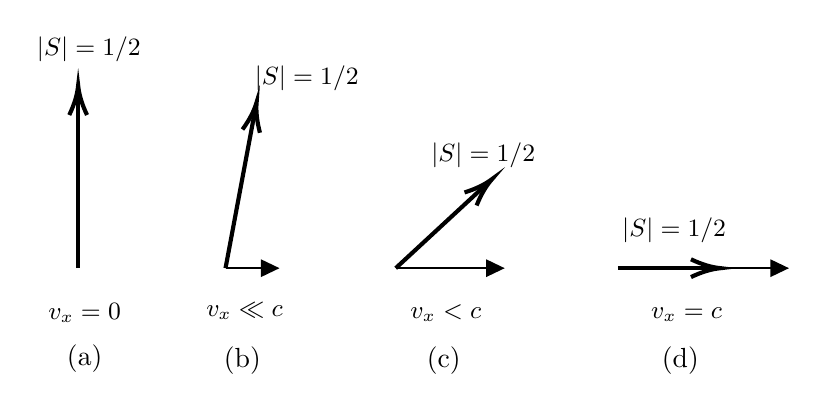
\begin{tikzpicture}[x=0.75pt,y=0.75pt,yscale=-1,xscale=1]
%uncomment if require: \path (0,300); %set diagram left start at 0, and has height of 300

%Straight Lines [id:da533603137195499] 
\draw [line width=1.5]    (79.87,190.5) -- (79.87,105.5) ;
\draw [shift={(79.87,102.5)}, rotate = 450] [color={rgb, 255:red, 0; green, 0; blue, 0 }  ][line width=1.5]    (14.21,-4.28) .. controls (9.04,-1.82) and (4.3,-0.39) .. (0,0) .. controls (4.3,0.39) and (9.04,1.82) .. (14.21,4.28)   ;

%Straight Lines [id:da31466198885223695] 
\draw    (150.87,190.5) -- (173.87,190.5) ;
\draw [shift={(176.87,190.5)}, rotate = 180] [fill={rgb, 255:red, 0; green, 0; blue, 0 }  ][line width=0.08]  [draw opacity=0] (8.93,-4.29) -- (0,0) -- (8.93,4.29) -- cycle    ;

%Straight Lines [id:da6431925700861189] 
\draw [line width=1.5]    (150.87,190.5) -- (165.31,113.45) ;
\draw [shift={(165.87,110.5)}, rotate = 460.62] [color={rgb, 255:red, 0; green, 0; blue, 0 }  ][line width=1.5]    (14.21,-4.28) .. controls (9.04,-1.82) and (4.3,-0.39) .. (0,0) .. controls (4.3,0.39) and (9.04,1.82) .. (14.21,4.28)   ;

%Straight Lines [id:da8282450907912188] 
\draw    (232.87,190.5) -- (282.37,190.5) ;
\draw [shift={(285.37,190.5)}, rotate = 180] [fill={rgb, 255:red, 0; green, 0; blue, 0 }  ][line width=0.08]  [draw opacity=0] (8.93,-4.29) -- (0,0) -- (8.93,4.29) -- cycle    ;

%Straight Lines [id:da09697600465348566] 
\draw [line width=1.5]    (232.87,190.5) -- (277.16,149.54) ;
\draw [shift={(279.37,147.5)}, rotate = 497.24] [color={rgb, 255:red, 0; green, 0; blue, 0 }  ][line width=1.5]    (14.21,-4.28) .. controls (9.04,-1.82) and (4.3,-0.39) .. (0,0) .. controls (4.3,0.39) and (9.04,1.82) .. (14.21,4.28)   ;

%Straight Lines [id:da13695386046952507] 
\draw    (339.87,190.5) -- (419.33,190.5) ;
\draw [shift={(422.33,190.5)}, rotate = 180] [fill={rgb, 255:red, 0; green, 0; blue, 0 }  ][line width=0.08]  [draw opacity=0] (8.93,-4.29) -- (0,0) -- (8.93,4.29) -- cycle    ;

%Straight Lines [id:da04790853968035602] 
\draw [line width=1.5]    (339.87,190.5) -- (386.33,190.5) ;
\draw [shift={(389.33,190.5)}, rotate = 180] [color={rgb, 255:red, 0; green, 0; blue, 0 }  ][line width=1.5]    (14.21,-4.28) .. controls (9.04,-1.82) and (4.3,-0.39) .. (0,0) .. controls (4.3,0.39) and (9.04,1.82) .. (14.21,4.28)   ;


% Text Node
\draw (85,85.07) node  [font=\small]  {$|S|=1/2$};
% Text Node
\draw (83,212.07) node  [font=\small]  {$v_{x} =0$};
% Text Node
\draw (160,211.07) node  [font=\small]  {$v_{x} \ll c$};
% Text Node
\draw (257,212.07) node  [font=\small]  {$v_{x} < c$};
% Text Node
\draw (373,213.07) node  [font=\small]  {$v_{x} =c$};
% Text Node
\draw (190,99.07) node  [font=\small]  {$|S|=1/2$};
% Text Node
\draw (275,136.07) node  [font=\small]  {$|S|=1/2$};
% Text Node
\draw (367,172.07) node  [font=\small]  {$|S|=1/2$};
% Text Node
\draw (83,234.07) node   [align=left] {(a)};
% Text Node
\draw (159,235.07) node   [align=left] {(b)};
% Text Node
\draw (256,235.07) node   [align=left] {(c)};
% Text Node
\draw (370,235.07) node   [align=left] {(d)};


\end{tikzpicture}

    \caption{Effect of Transverse Velocity on Dirac Particle Spin}
    \label{fig:transverse-velocity-effect}
\end{figure}

In general, for $j=a,b,c,d$, the four states shown (for a C type particle) in the figure are
\begin{equation}
\left|\psi_{(j)}\right\rangle=\sqrt{\frac{m}{V E_{p_{j}}}}\left(C_{1}\left(p_{j}\right) u_{1}\left(p_{j}\right)+C_{2}\left(p_{j}\right) u_{2}\left(p_{j}\right)\right) e^{-i p_{j} x}
\label{psi-abcd}
\end{equation}
Not that we have a particle here (so no $D$ type terms), and $\mathbf{p}_j$ is known. State (a) there is effectively spin up with $\mathrm{p}_{\mathrm{a}}=0$, so
\begin{equation}
\left|\psi_{(a)}\right\rangle=\sqrt{\frac{m}{V E_{p_{a}}}} C_{1}(0) u_{1}(0) e^{-i p_{a} x}=\sqrt{\frac{m}{V E_{\mathrm{p}_{a}}}} \sqrt{\frac{E_{\mathrm{p}_{a}}+m}{2 m}}\left(\begin{array}{l}
{\mathrm{I}} \\
{0} \\
{0} \\
{0}
\end{array}\right) e^{-i p_{a} x}
\end{equation}
which is an eigenstate of $\Sigma_3$. So for state (a), $|\psi_a\rangle$ has $C_1=1$ and $C_2=0$.

For the last state (d), where the particle is traveling at the speed of light, (\ref{psi-abcd}) becomes an eigenstate of $\Sigma_1$ with eigenvalue $1/2$,
$$
\left|\psi_{(d)}\right\rangle=\sqrt{\frac{m}{V E_{\mathrm{p}_{d}}}} C_{1}(\infty) u_{1}(\infty) e^{-i p_{d} x}+\sqrt{\frac{m}{V E_{\mathrm{p} d}}} C_{2}(\infty) u_{2}(\infty) e^{-i p_{d} x}
$$
$$
=\sqrt{\frac{m}{V E_{\mathrm{p}_{d}}}} \sqrt{\frac{E_{\mathrm{p}_{d}}+m}{2 m}}\left(\begin{array}{l}
{1} \\
{1} \\
{1} \\
{1}
\end{array}\right) e^{-i p_{d} x}
$$
where here, we must have $C_1=C_2=1$. (in the normalized version, $C_1=C_2=1/\sqrt{2}$).For "in between" states $(b)$ and $(c), C_{1}$ and $C_{2}$ would have other values. The bottumline is:\redp{$\mathbf{p}$ determines $u_{1,2}$ and then spin is represented by correct linear combination of $u_1$ and $u_2$}. Note that \bluep{we can never have a relativistic state where the spin vector and $\mathbf{p}$ are at right angles.}

Note that $u_{1}$ and $u_{2}$ actually exist in spinor space (they are spinor space basis vectors in that space), but they correspond to directions in physical space. For example, in the at-rest system, $u_1$ represents spin up and so can be visualized as a spatial vector that points in the $+z$ direction. Similarly, in the at-rest system, $u_{2}$ represents spin down, so can be visualized as a vector pointing in the $-z$ direction. 
\begin{qt}
\underline{Summary}

1. $\left.u_{1}(\mathrm{p}) e^{-i p x} \text { and } u_{2}(\mathrm{p}) e^{-i p x} \text { is each always an eigenstate of the Dirac equation (for any } \mathbf{p}\right)$

2. $u_{1}(\mathrm{p}) e^{-i p x}$ and $u_{2}(\mathrm{p}) e^{-i p x}$ is each sometimes an eigenstate of $z$ spin, i.e. of $\Sigma_{3}\left(\text { for } \mathbf{p}=0 \text { or }=p^{3} \mathbf{i}_{3}\right)$

3. $u_{1}(\mathbf{p}) e^{-i p x}$ and $u_{2}(\mathbf{p}) e^{-i p x}$ are always basis vectors for any general state $|\psi\rangle$ (for any $\mathbf{p}$ )

4. $u_{1}(p)$ and $u_{2}(p)$ is each sometimes an eigenstate of $z$ spin, i.e. of $\Sigma_{3}\left(\text { for } \mathbf{p}=0 \text { or }=p^{3} \mathbf{i}_{3}\right)$

5. $u_{1}(\mathbf{p})$ and $u_{2}(\mathbf{p})$ are always basis vectors in $4 \mathrm{D}$ spinor space (for any $\mathbf{p}$) 

6.\textbf{$u_{1}(\mathrm{p})$ and $u_{2}(\mathrm{p})$ change orientation, as visualized in physical space, as $\mathrm{p}$ changes.}

7. Spin S (often in relativity as $\Sigma$ ) changes direction with p, but differently than $u_{1}$ and $u_{2}$
\end{qt}
Any general spin state $u$ can be represented as a linear combination of $u_{1}$ and  $u_{2}$ (for any $\mathbf{p}$ )
$$
u(\mathrm{p})=C_{1}(\mathrm{p}) u_{1}(\mathrm{p})+C_{2}(\mathrm{p}) u_{2}(\mathrm{p})
$$
Any general particle state includes a spin part plus a spacetime part(for any given $\mathbf{p}$):
$$
\left|\psi_{\mathfrak{p}}\right\rangle=\sqrt{\frac{m}{2 V E_{\mathrm{p}}}} u(\mathbf{p}) e^{-i p x}=\sqrt{\frac{m}{2 V E_{\mathrm{p}}}}\left(C_{1}(\mathrm{p}) u_{1}(\mathrm{p}) e^{-i p x}+C_{2}(\mathrm{p}) u_{2}(\mathrm{p}) e^{-i p x}\right)
$$